\documentclass{beamer}

\mode<presentation> {
\usetheme{Madrid}
}
\newtheorem{definition}{Definition}
\newtheorem{proposition}{Proposition}
\usepackage{amsmath}
\usepackage{algorithm}
\newcommand{\isometrypursuit}{{\sc IsometryPursuit}}
\usepackage[font=small]{caption}
\captionsetup[algorithm]{labelformat=empty}
% \usepackage{algpseudocode}
\usepackage{algorithmic}

%\bibliography{ref}
% \AtEveryCitekey{\renewcommand{\multicitedelim}{\newline}\clearfield{pages}}
%\makeatletter
%\DeclareCiteCommand{\fullcite}
 % {\usebibmacro{prenote}}
 % {\usedriver
 %    {\DeclareNameAlias{sortname}{default}}
 %    {\thefield{entrytype}}\par\setunit{\bibsentence}\newblock\par\medskip}
%  {}
%  {\usebibmacro{postnote}}
%\makeatother



\title[]{Isometry pursuit}
\author[Koelle, S.J.]{
Samson Koelle} %

\begin{document}

{
\usebackgroundtemplate{\includegraphics[width=\paperwidth]{img/ant.jpg}}
\begin{frame}
\titlepage 
\end{frame}
}

%\begin{frame}{The problem}
\small
\begin{columns}
\begin{column}{0.5\textwidth}
\begin{figure}[h!]
    \centering
    \includegraphics[width=0.8\linewidth]{img/snoots.png} % Replace 'filename.jpg' with your image file
\end{figure}

\vspace{-.5cm}
\end{column}
\begin{column}{0.5\textwidth}
\begin{figure}[h!]
    \centering
    \includegraphics[width=1.\linewidth]{../figures/interpretabledirections.png} % Replace 'filename.jpg' with your image file
\end{figure}
\vspace{-.5cm}
\end{column}
\end{columns}
\end{frame}

\begin{frame}{Isometry selection}
\small

\begin{figure}[h!]
    \centering
    \includegraphics[width=.6\linewidth]{../figures/goldencompass.png} % Replace 'filename.jpg' with your image file
\end{figure}

\end{frame}

\begin{frame}{Yet another matrix loss}
\small
\begin{columns}
\begin{column}{0.5\textwidth}
Given a rank $D$ matrix $X \in \mathbb{R}^{D \times P}$ with singular values $\sigma_d \in [D]$, let
\begin{align*}
\ell_{c}: \mathbb{R}^{D \times P} &\to \mathbb{R}^+ \\
X &\mapsto \sum_{d=1}^D g(\sigma_d(X), c) - D\\
\\[-1ex]
g: \mathbb{R}^+ \times \mathbb{R}^+ &\to \mathbb{R}^+ \\
(t, c) &\mapsto \frac{e^{t^c} + e^{t^{-c}}}{2e}.
\end{align*}
\vspace{-.5cm}
\end{column}
\begin{column}{0.5\textwidth}
\begin{figure}[h!]
    \centering
    \includegraphics[width=.6\linewidth]{../figures/Figure_1a_ct} % Replace 'filename.jpg' with your image file
\end{figure}
\begin{figure}[h!]
    \centering
    \includegraphics[width=.6\linewidth]{../figures/isometree} % Replace 'filename.jpg' with your image file
\end{figure}
\end{column}
\end{columns}
\end{frame}




%\begin{frame}
%\frametitle{Sections} 
% \tableofcontents 
%\end{frame}

%\section{Background and motivation}
\begin{frame}{The problem}
\small
\begin{columns}
\begin{column}{0.5\textwidth}
\begin{figure}[h!]
    \centering
    \includegraphics[width=0.8\linewidth]{img/snoots.png} % Replace 'filename.jpg' with your image file
\end{figure}

\vspace{-.5cm}
\end{column}
\begin{column}{0.5\textwidth}
\begin{figure}[h!]
    \centering
    \includegraphics[width=1.\linewidth]{../figures/interpretabledirections.png} % Replace 'filename.jpg' with your image file
\end{figure}
\vspace{-.5cm}
\end{column}
\end{columns}
\end{frame}

\begin{frame}{Isometry selection}
\small

\begin{figure}[h!]
    \centering
    \includegraphics[width=.6\linewidth]{../figures/goldencompass.png} % Replace 'filename.jpg' with your image file
\end{figure}

\end{frame}

\begin{frame}{Yet another matrix loss}
\small
\begin{columns}
\begin{column}{0.5\textwidth}
Given a rank $D$ matrix $X \in \mathbb{R}^{D \times P}$ with singular values $\sigma_d \in [D]$, let
\begin{align*}
\ell_{c}: \mathbb{R}^{D \times P} &\to \mathbb{R}^+ \\
X &\mapsto \sum_{d=1}^D g(\sigma_d(X), c) - D\\
\\[-1ex]
g: \mathbb{R}^+ \times \mathbb{R}^+ &\to \mathbb{R}^+ \\
(t, c) &\mapsto \frac{e^{t^c} + e^{t^{-c}}}{2e}.
\end{align*}
\vspace{-.5cm}
\end{column}
\begin{column}{0.5\textwidth}
\begin{figure}[h!]
    \centering
    \includegraphics[width=.6\linewidth]{../figures/Figure_1a_ct} % Replace 'filename.jpg' with your image file
\end{figure}
\begin{figure}[h!]
    \centering
    \includegraphics[width=.6\linewidth]{../figures/isometree} % Replace 'filename.jpg' with your image file
\end{figure}
\end{column}
\end{columns}
\end{frame}




\section{Background}

In this section, we give background on the isometry and diversification problems, as well as the spectral and convex analysis that motivate our method.

\subsection{Problem}

Our goal is, given a matrix $ X \in \mathbb R^{D \times P}$, to select a subset $ S \subset [P]$ with $| S| = D$ such that $X_{.  S}$ is as orthonormal as possible in a computationally efficient way.
% To this end, we define a ground truth loss function that measures orthonormalness, and then introduce a surrogate loss function that convexifies the problem.

\subsection{Interpretability and isometry}

One motivating example is the selection of data representations from within sets of putative coordinates: the columns of a provided wide matrix.
This method applies to interpretability, for which parsimony is at a premium.
Interpretability arises through comparison of data with what is known to be important in the domain of the problem.
This knowledge often takes the form of a functional dictionary.
Evaluation of independence of dictionary features arises in numerous scenarios \citep{Chen2019-km, Koelle2022-ju, He2023-ch}.
The requirement that dictionary features be full rank has been called functional independence \citep{Koelle2022-ju} or feature decomposability \citep{templeton2024scaling}, with connection between dictionary rank and independence via the implicit function theorem.
Besides independence, the metric properties of such dictionary elements are of natural interest.
This is formalized through the notion of differential.

\begin{definition}
The \textbf{differential} of a smooth map $\phi:\mathcal M \to \mathcal N$ between $D$ dimensional manifolds $\M \subseteq \mathbb R^B$ and $\N \subseteq \mathbb R^P$ is a map in tangent bases $x_1 \dots x_{D}$ of $T_\xi \M$ and $y_1 \dots y_{D}$ of $T_{\phi(\xi)} \N$ consisting of entries
\begin{align}
\label{eq:diff}
    D\phi (\xi) = \begin{bmatrix}
    \frac{\partial \phi_1  }{\partial x_1}(\xi)  & \dots & \frac{\partial \phi_1 }{\partial x_D}(\xi)  \\
    \vdots & & \vdots \\
    \frac{\partial \phi_D }{\partial x_1}(\xi)  & \dots & \frac{\partial \phi_{D}  }{\partial x_{D}}(\xi) 
    \end{bmatrix}.
\end{align}
\end{definition}

It is not always necessary to explicitly estimate tangent spaces when applying this definition.
The most commonly encountered manifolds are vector spaces for which the tangent spaces are trivial.
This is the case for full-rank tabular data, for which isometry has a natural interpretation as a type of diversification, and often for the latent spaces of deep learning models.
In this case, $B = D$.

\begin{definition}
\label{def:isometric_at_a_point}
A map $\phi$ between $D$ dimensional submanifolds with inherited Euclidean metric $\mathcal M \subseteq R^{B}$ and $\mathcal N  \subseteq R^{P}$
$\phi$ is an \textbf{isometry at a point} $\xi \in \mathcal M$ if
\begin{align}
{D \phi (\xi)}^T D \phi (\xi) = I_D.
\end{align}
That is, $\phi$ is an isometry at $\xi$ if $D \phi (\xi)$ is orthonormal.
\end{definition}

The applications of pointwise isometry are themselves manifold.
Pointwise isometric embeddings faithfully preserve high-dimensional geometry.
For example, Local Tangent Space Alignment \citep{ZhangZ:04}, Multidimensional Scaling \citep{ChenBuja:localMDS09} and Isomap \citep{tenenbaum2000ggf} non-parametrically estimate embeddings that are as isometric as possible.
Another approach stitches together pointwise isometries selected from a dictionary to form global embeddings \citep{Kohli2021-lr}.
The method is particularly relevant since it constructs such isometries through greedy search, with putative dictionary features added one at a time.

That $D\phi$ is orthonormal has several equivalent formulations.
The one motivating our ground truth loss function comes from spectral analysis.
\begin{proposition}
\label{prop:orthonormal_spectrum}
The singular values $\sigma_1 \dots \sigma_D$ are equal to $1$ if and only if $U \in \mathbb{R}^{D \times D}$ is orthonormal.
\end{proposition}
On the other hand, the formulation that motivates our convex approach is that orthonormal matrices consist of $D$ coordinate features whose gradients are orthogonal and of unit length.
\begin{proposition}
\label{prop:orthonormal_basis}
The component vectors $u_1 \dots u_D \in \mathbb R^B$ form a orthonormal matrix if and only if, for all $d_1, d_2 \in [D], \langle u_{d_1}, u_{d_2} \rangle = \begin{cases}
1 \; d_1 = d_2 \\ 
0 \; d_1 \neq d_2 
\end{cases}$.
\end{proposition}

\subsection{Diversification}

Cosine
MMR definition.
Embeddings - sim is just projection

\subsection{Best subset selection}

Given a matrix $ X \in \mathbb R^{D \times P}$, we compare algorithmic paradigms for solving problems of the form
\begin{align}
\label{prog:ground_truth}
\arg \min_{ S \in \binom{[P]}{D}} l ( X_{. S})
\end{align}
where $\binom{[P]}{D} = \left\{ A \subseteq [P] : \left|A\right| = D \right\}$.
Brute force algorithms consider all possible solutions.
These algorithms are conceptually simple, but have the often prohibitive time complexity $O(C_lP^D)$ where $C_l$ is the cost of evaluating $l$.
Greedy algorithms consist of iteratively adding one element at a time to $ S$.
This algorithms have time complexity $O(C_lPD)$ and so are computationally more efficient than brute force algorithms, but can get stuck in local minima.
Formal definitions are given in Section \ref{sec:algorithms}.

Sometimes, it is possible to introduce an objective which convexifies problems of the above form.
Solutions
\begin{align}
\arg \min f(\beta) : Y  = X\beta 
\end{align}
to the overcomplete regression problem $Y = X \beta$ are a classic example \citep{Chen2001-hh}.
When $f(\beta) = \|\beta\|_0$, this problem is non-convex, and is thus suitable for greedy or brute algorithms, but when $f(\beta) =\|\beta\|_1$, the problem is convex, and may be solved efficiently via interior-point methods.
When the equality constraint is relaxed, Lagrangian duality may be used to reformulate as a so-called Lasso problem, which leads to an even richer set of optimization algorithms. % cite FISTA< glmnet, coordinate descent

The form of basis pursuit that we apply is inspired by the group basis pursuit approach in \citet{Koelle2022-ju}.
In group basis pursuit (which we call multitask basis pursuit when grouping is dependent only on the structure of matrix-valued response variable $y$) the objective function is $f(\beta) = \|\beta\|_{1,2} := \sum_{p=1}^P \|\beta_{p.}\|_2$  \citep{Yuan2006-bt, Obozinski2006-kq, Yeung2011-fg}.
This objective creates joint sparsity across entire rows $\beta_{p.}$ and was used in \citet{Koelle2022-ju} to select between sets of interpretable features.
%\section{Algorithm and results}
%
\begin{frame}{Dictionary-based manifold learning}
\begin{algorithm}[H]
\caption{\tsalg(Dataset $\mathcal D$, dictionary $g$)}
\begin{algorithmic}[1]
\STATE Compute Jacobian $d g (n) \in \mathbb R^{P \times B} \; \forall  n \in [N]$
\STATE Normalize $\|d g^p \|_F = \sqrt{N} \; \forall  p \in [P]$
\STATE Estimate tangent basis $T_{\mathcal M}(n) \in \mathbb R^{D \times B} \; \forall  n \in [N]$
\STATE Project $d_\M g (n) = {T_{\mathcal M} (n)}^T d g (n) \; \forall  n \in [N]$
\STATE  $\hat \beta \gets \arg \min_{\beta \in \mathbb R^{N \times P \times D}} J_\lambda ( d_\M g ([N]),\beta)$ (Group Lasso)
\STATE {\bf Output} $S= \supp \hat  \beta$ 
\end{algorithmic}
\end{algorithm}
\begin{itemize}
\item $J_\lambda (X, \beta) =  \frac{1}{2}\sum_{n=1}^N \| I_D  - X_{n..} \beta_{n..}\|_F^2+\frac{\lambda}{\sqrt{DN}} \sum_{p=1}^P \|\beta_{.p.}\|_F. $
\item Optimize with FISTA
\item Locate region on regularization path with $|S| = D$ using binary search
\end{itemize}
\end{frame}


\begin{frame}{Estimating tangent spaces using local PCA}
\begin{columns}
\begin{column}{0.35\textwidth}
\begin{itemize}
    \item First, perform a nearest neighbor search around $\xi = \mathcal D(n) \in \mathcal M$
    \item Then, estimate $ T_{\mathcal M}(n) $ using the top singular vectors $[x^1, \dotsc x^D]$ of the centered neighbors
\end{itemize}
\end{column}
\begin{column}{0.6\textwidth}
\begin{figure}
    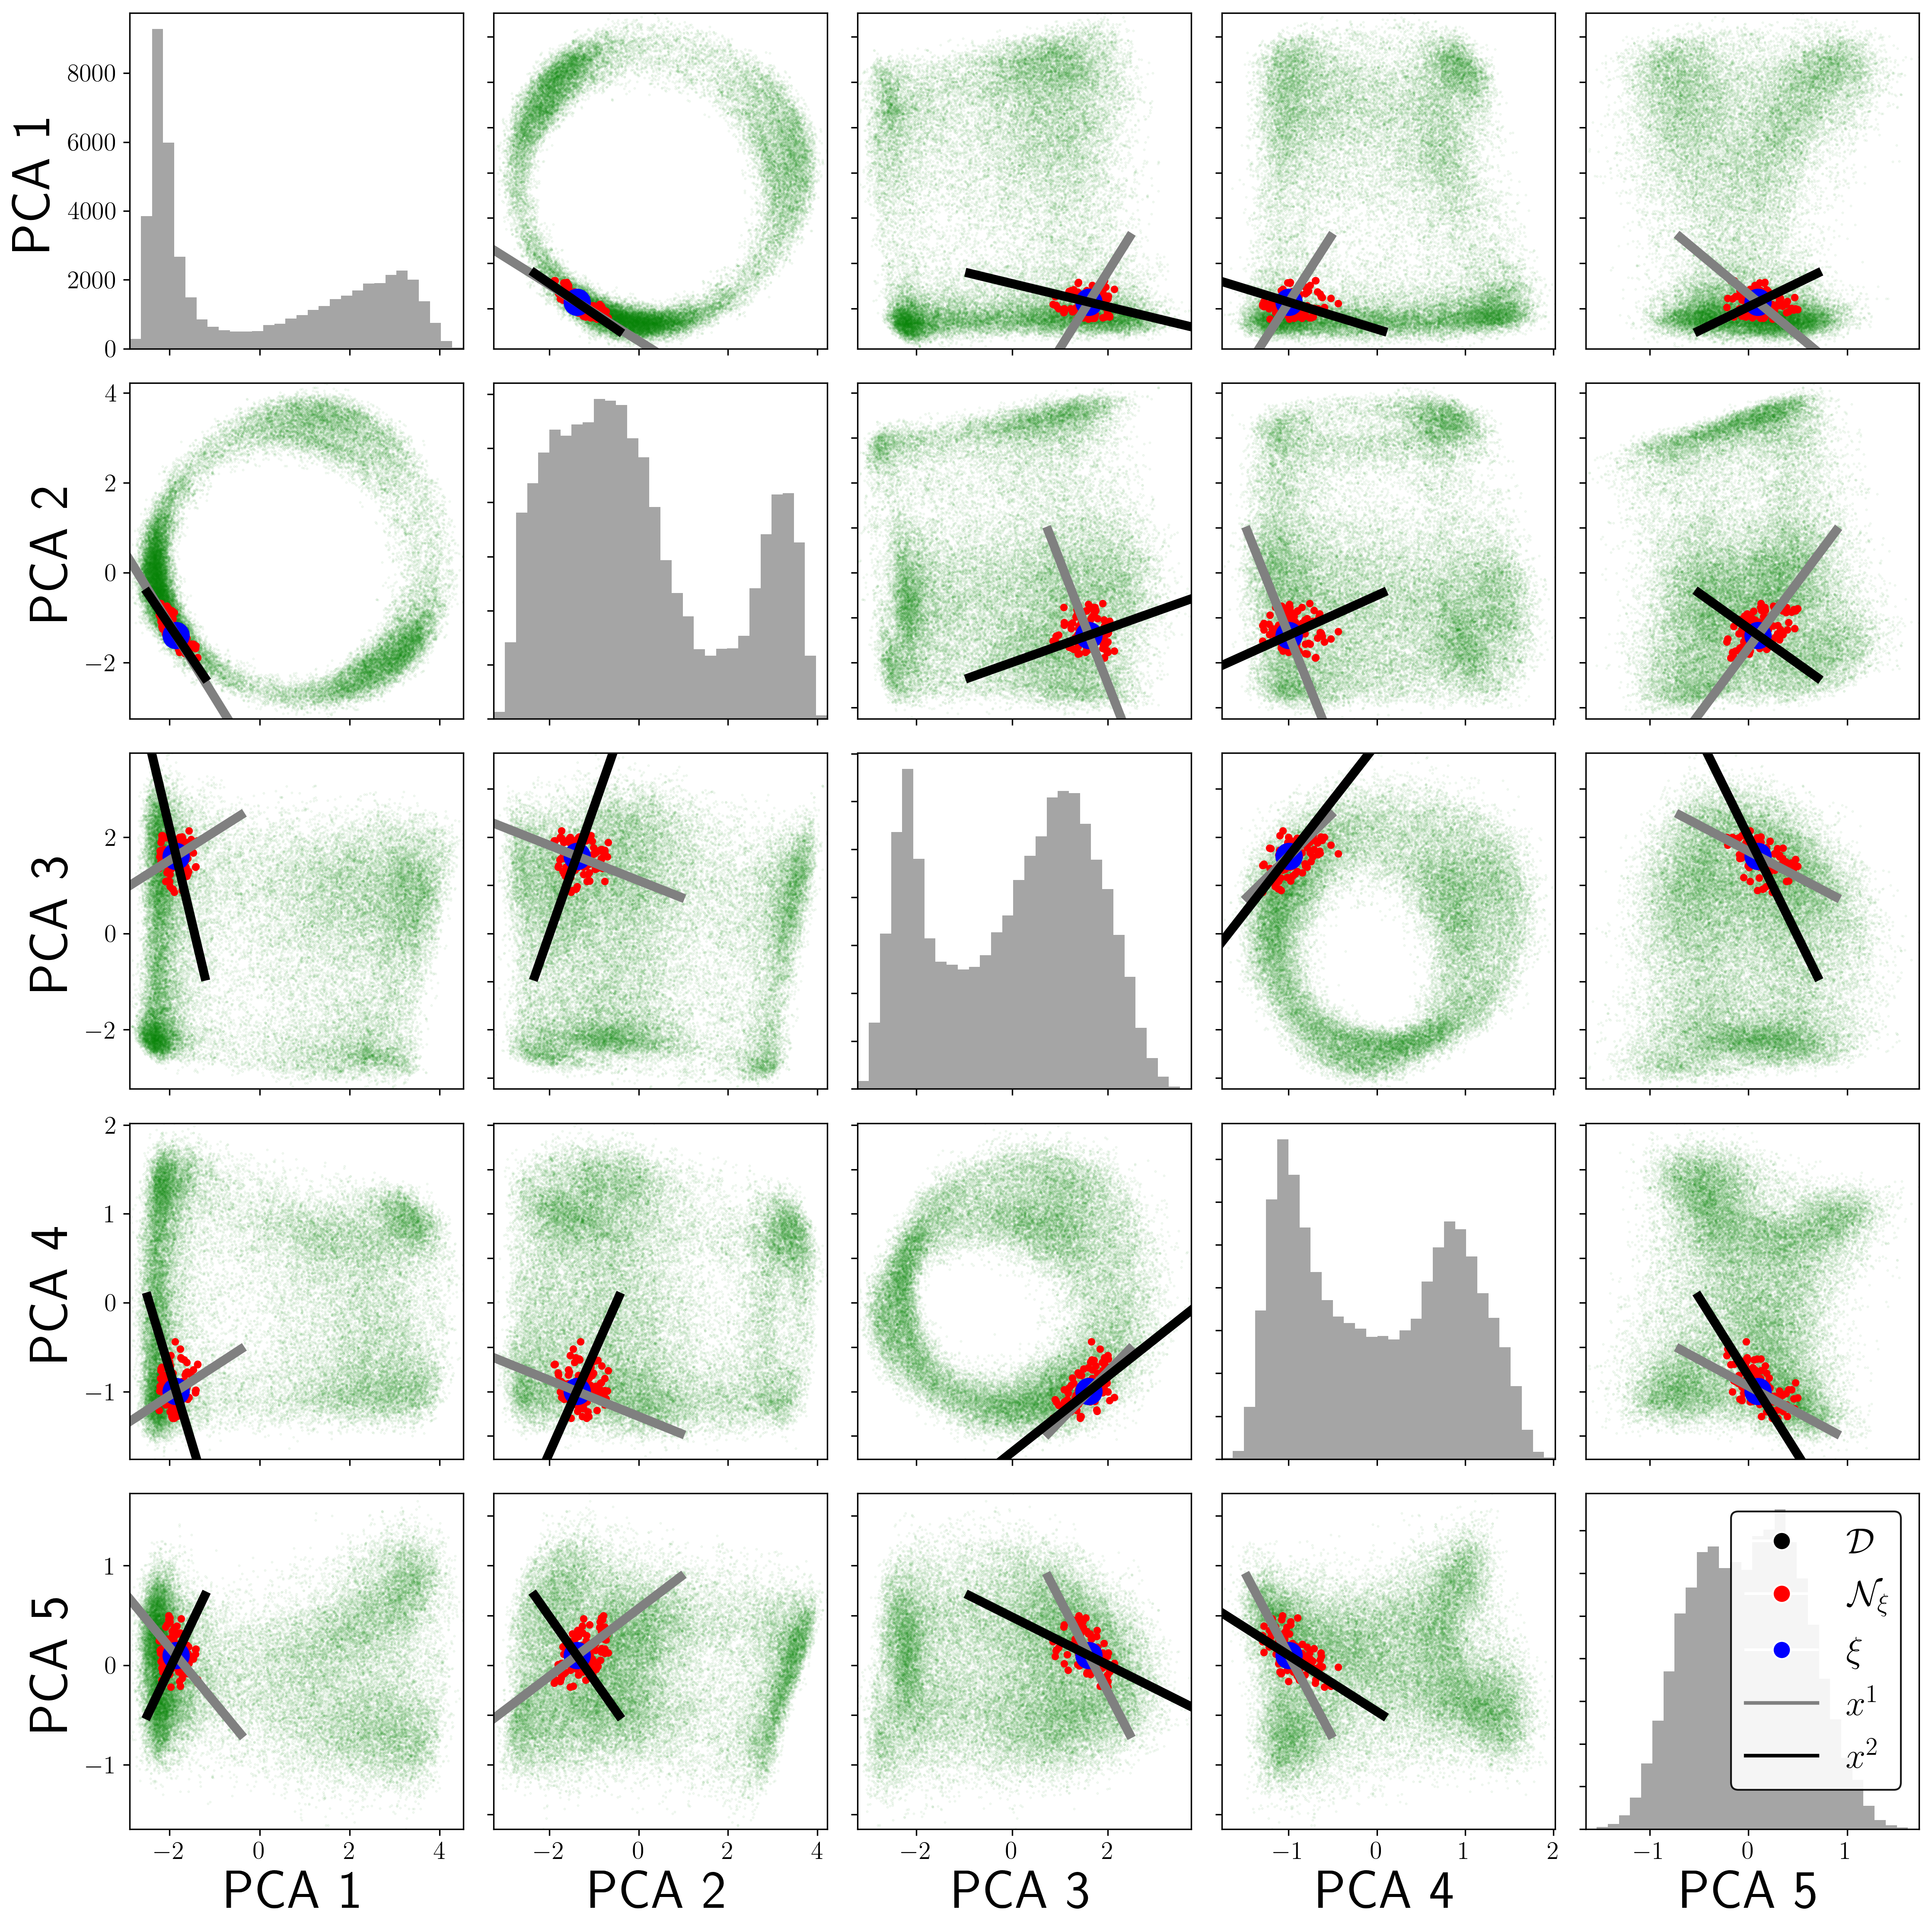
\includegraphics[width=2.5in]{img/tangentspaces.png}
    \caption*{A neighborhood and tangent space plotted in top global PCA coordinates}
\end{figure}
\end{column}
\end{columns}


\end{frame}

\begin{frame}{Gradients}
\begin{itemize}
    \item We can compute dihedral angle gradients with autograd
    \item We then project $d_{\mathcal M} g (n) = (T_{\mathcal M} (n))^T d g (n)$
\end{itemize}
\small
\begin{figure}[!htp]
    \centering
    \begin{tabular}{p{2.5cm}p{2.5cm}p{2.5cm}p{2.5cm}}
        \includegraphics[width=0.25\textwidth, trim={2cm 3cm 5cm 0cm}, clip]{img/ethanol_g0.png} &
        \includegraphics[width=0.25\textwidth, trim={2cm 3cm 5cm 0cm}, clip]{img/ethanol_g1.png} &
          \includegraphics[width=0.25\textwidth, trim={2cm 3cm 5cm 0cm}, clip]{img/ethanol_g2.png} &
          \includegraphics[width=0.25\textwidth, trim={2cm 3cm 5cm 0cm}, clip]{img/ethanol_g3.png}  \\
        \includegraphics[width=0.2\textwidth]{img/tangent_0.png} &
        \includegraphics[width=0.2\textwidth]{img/tangent_1.png} &
         \includegraphics[width=0.2\textwidth]{img/tangent_2.png}  &
          \includegraphics[width=0.2\textwidth]{img/tangent_3.png} 
    \end{tabular}
    %\vspace{-2cm}
    \caption*{ Gradients $dg^p = \frac{\partial g^p }{\partial x^d} $ of four dihedral angles $g^p:\mathcal M \to \mathbb R$ with respect to coordinates $x^1 \dots x^D$ of tangent space $\mathcal {T}_{\mathcal M} (n)$}
\end{figure}
\end{frame}


\begin{frame}{Normalization}
\begin{itemize}
    \item We normalize $d g^p(n)= \frac{\sqrt{N} d g^p(n)}{  \|d g^p([N])\|_F}$ prior to projection to favor gradient fields which are more tangent to the manifold
\end{itemize}
\begin{figure}[!htp]
    \centering
    \begin{tabular}{ccc}
        \includegraphics[width=0.3\textwidth, trim={3cm 2cm 5cm 3cm}, clip]{img/raw.png} &
        \includegraphics[width=0.3\textwidth, trim={3cm 2cm 5cm 3cm}, clip]{img/norm.png} &
          \includegraphics[width=0.3\textwidth, trim={3cm 2cm 5cm 3cm}, clip]{img/proj.png}  \\
           \centering
        $dg$ &
         \centering
       $dg$ (normalized) &
        \centering
        $d_{\mathcal M} g$
    \end{tabular}
    \caption*{Gradients of example functions \textcolor{red}{$g^1$} and \textcolor{blue}{$g^2$} for $B = 2, D = 1$}
\end{figure}
\begin{itemize}
    \item Note: gradients of dihedral angles w.r.t. planar angles are not well-defined and so we use $dg = d_{\mathbb R^{3N_a}} g (d_{\mathbb R^{3N_a}} \alpha)^{\dagger_{3N_a - 7}}$
\end{itemize}
\end{frame}

\begin{frame}{Results}
\begin{figure}[!htp]
    \centering
    \begin{tabular}{p{3cm}p{3cm}p{3cm}}
        \includegraphics[width=0.2\textwidth]{img/reg_small.png} &
        \includegraphics[width=0.35\textwidth, trim={3cm 0cm 0cm 4cm}, clip]{img/ethanol_g0.png} &
          \includegraphics[width=0.35\textwidth, trim={3cm 0cm 0cm 4cm}, clip]{img/ethanol_g2.png}  \\
        \includegraphics[width=0.2\textwidth, trim={0cm 0cm 3cm 0cm}, clip]{img/cosines_sellasso_small.png} &
        \includegraphics[width=0.35\textwidth, trim={3cm 0cm 0cm 3cm}, clip]{img/ethanol_small_embedding_0.png} &
          \includegraphics[width=0.35\textwidth, trim={3cm 0cm 0cm 3cm}, clip]{img/ethanol_small_embedding_1.png} 
    \end{tabular}
    %\vspace{-2cm}
    \caption*{Results for one replicate with $P=12$ dictionary functions implicitly defined by the ethanol bond diagram}
\end{figure}
\end{frame}
% 1 


%\begin{frame}{Thank you!}
%I'm happy to take any questions.
%\end{frame}

\end{document}


